\documentclass{article}
\usepackage{color}
\usepackage{amsmath, amssymb}
\usepackage{graphicx}
\usepackage{pdfpages}

\setlength{\textwidth}{6.5in}
\setlength{\textheight}{8.0in}
\setlength{\oddsidemargin}{0in}
\setlength{\evensidemargin}{0in}
\setlength{\parskip}{2ex}
\setlength{\parindent}{0in}

%To display answers, replace "white" with "red" here;
\newcommand{\answer}[1]{\color{red}#1}

\begin{document}
\pagestyle{myheadings}\markright{
CU Boulder \hspace{0.5in} MATH 2510 - Introduction to Statistics}

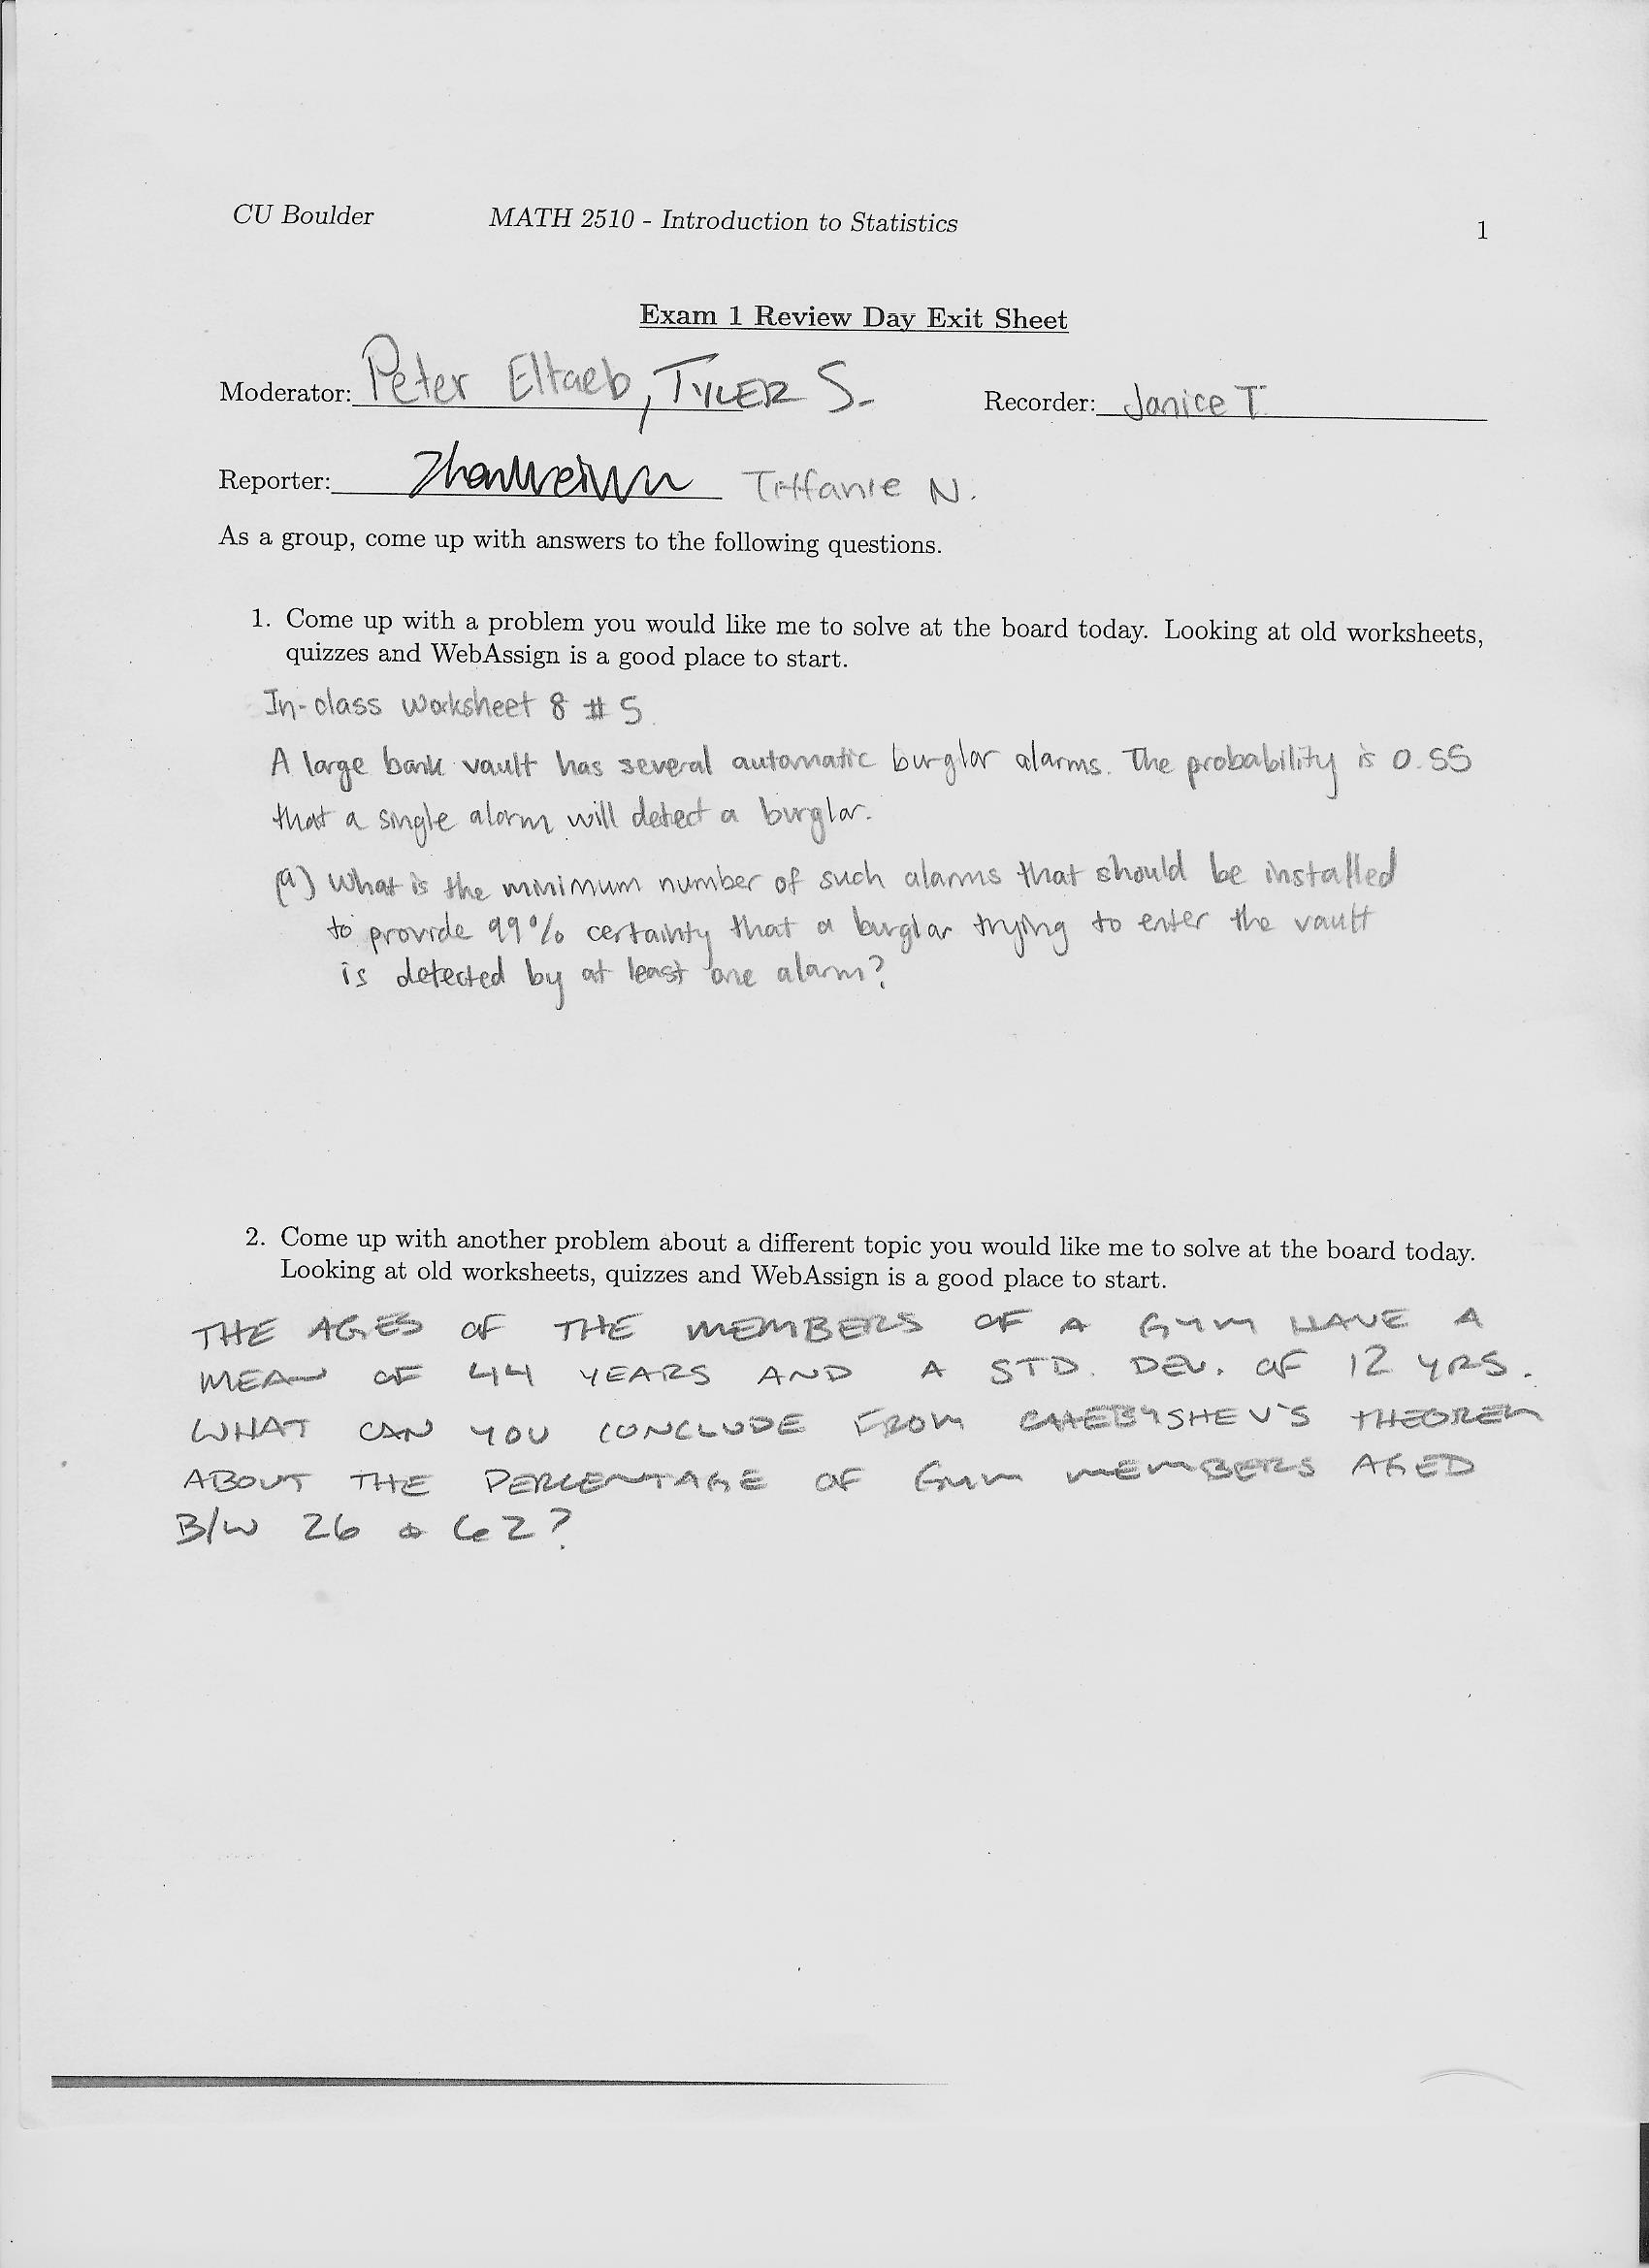
\includepdf{Exam1Exitsheet1.jpg}

\begin{center}
\textbf{\underbar{Exam 1 Review Day Exit Sheet}}
\end{center}

Moderator:{\underbar{\hspace{2in}}} \hfill  Recorder:{\underbar{\hspace{2in}} }

\bigskip

Reporter:{\underbar{\hspace{2in}}}

As a group, come up with answers to the following questions.

\begin{enumerate} 

\item Come up with a problem you would like me to solve at the board today. Looking at old worksheets, quizzes and WebAssign is a good place to start.

{\answer The goal of this problem is to find a $n$ large enough so that $P(X\geq 1) \geq 0.9$ where $X$ is a binomial random variable with an unknown $n$ number of trials and probability of a successful trial is 0.55.

One method is to guess and check (described in Worksheet 8 Solutions, problem 5a), the other method is to use logarithms (not required in this class).

$$P(X\geq 1) = 1- P(X=0) = 1- (1-0.55)^n = 1-(0.45)^n.$$

So we want 
\begin{align*}
0.99 &\geq 1- (0.45)^n \\
(0.45)^n \geq 0.01 \\
n \log 0.55 \geq \log 0.01 \\
n \geq \frac{\log 0.01}{\log 0.45} \approx 5.76722 \end{align*}

Since $n$ needs to be an integer, we round up to the answer of 6.}

\item Come up with another problem about a different topic you would like me to solve at the board today. Looking at old worksheets, quizzes and WebAssign is a good place to start. 

{\answer Chebyshev's theorem concerns intervals centered around the mean $(\mu)$ and its length is determined by a number of standard deviations $k$. So the first step is to verify this interval $(26,62)$ can be expressed as $\mu \pm k\sigma$.
$$62 = 44 + k(12) \Rightarrow k=1.5$$
$$26 = 44 - k(12) \Rightarrow k=1.5$$
So now we may apply Chebyshev's theorem, which will conclude that there is at least $\left(1-\frac{1}{k^2}\right) \%$ of the population (or data) falls within this range.
$$1-\frac{1}{(1.5)^2} = 0.5555555...$$
So we have at least 55.6\% of the gym members within this age range.}
\end{enumerate}

\newpage

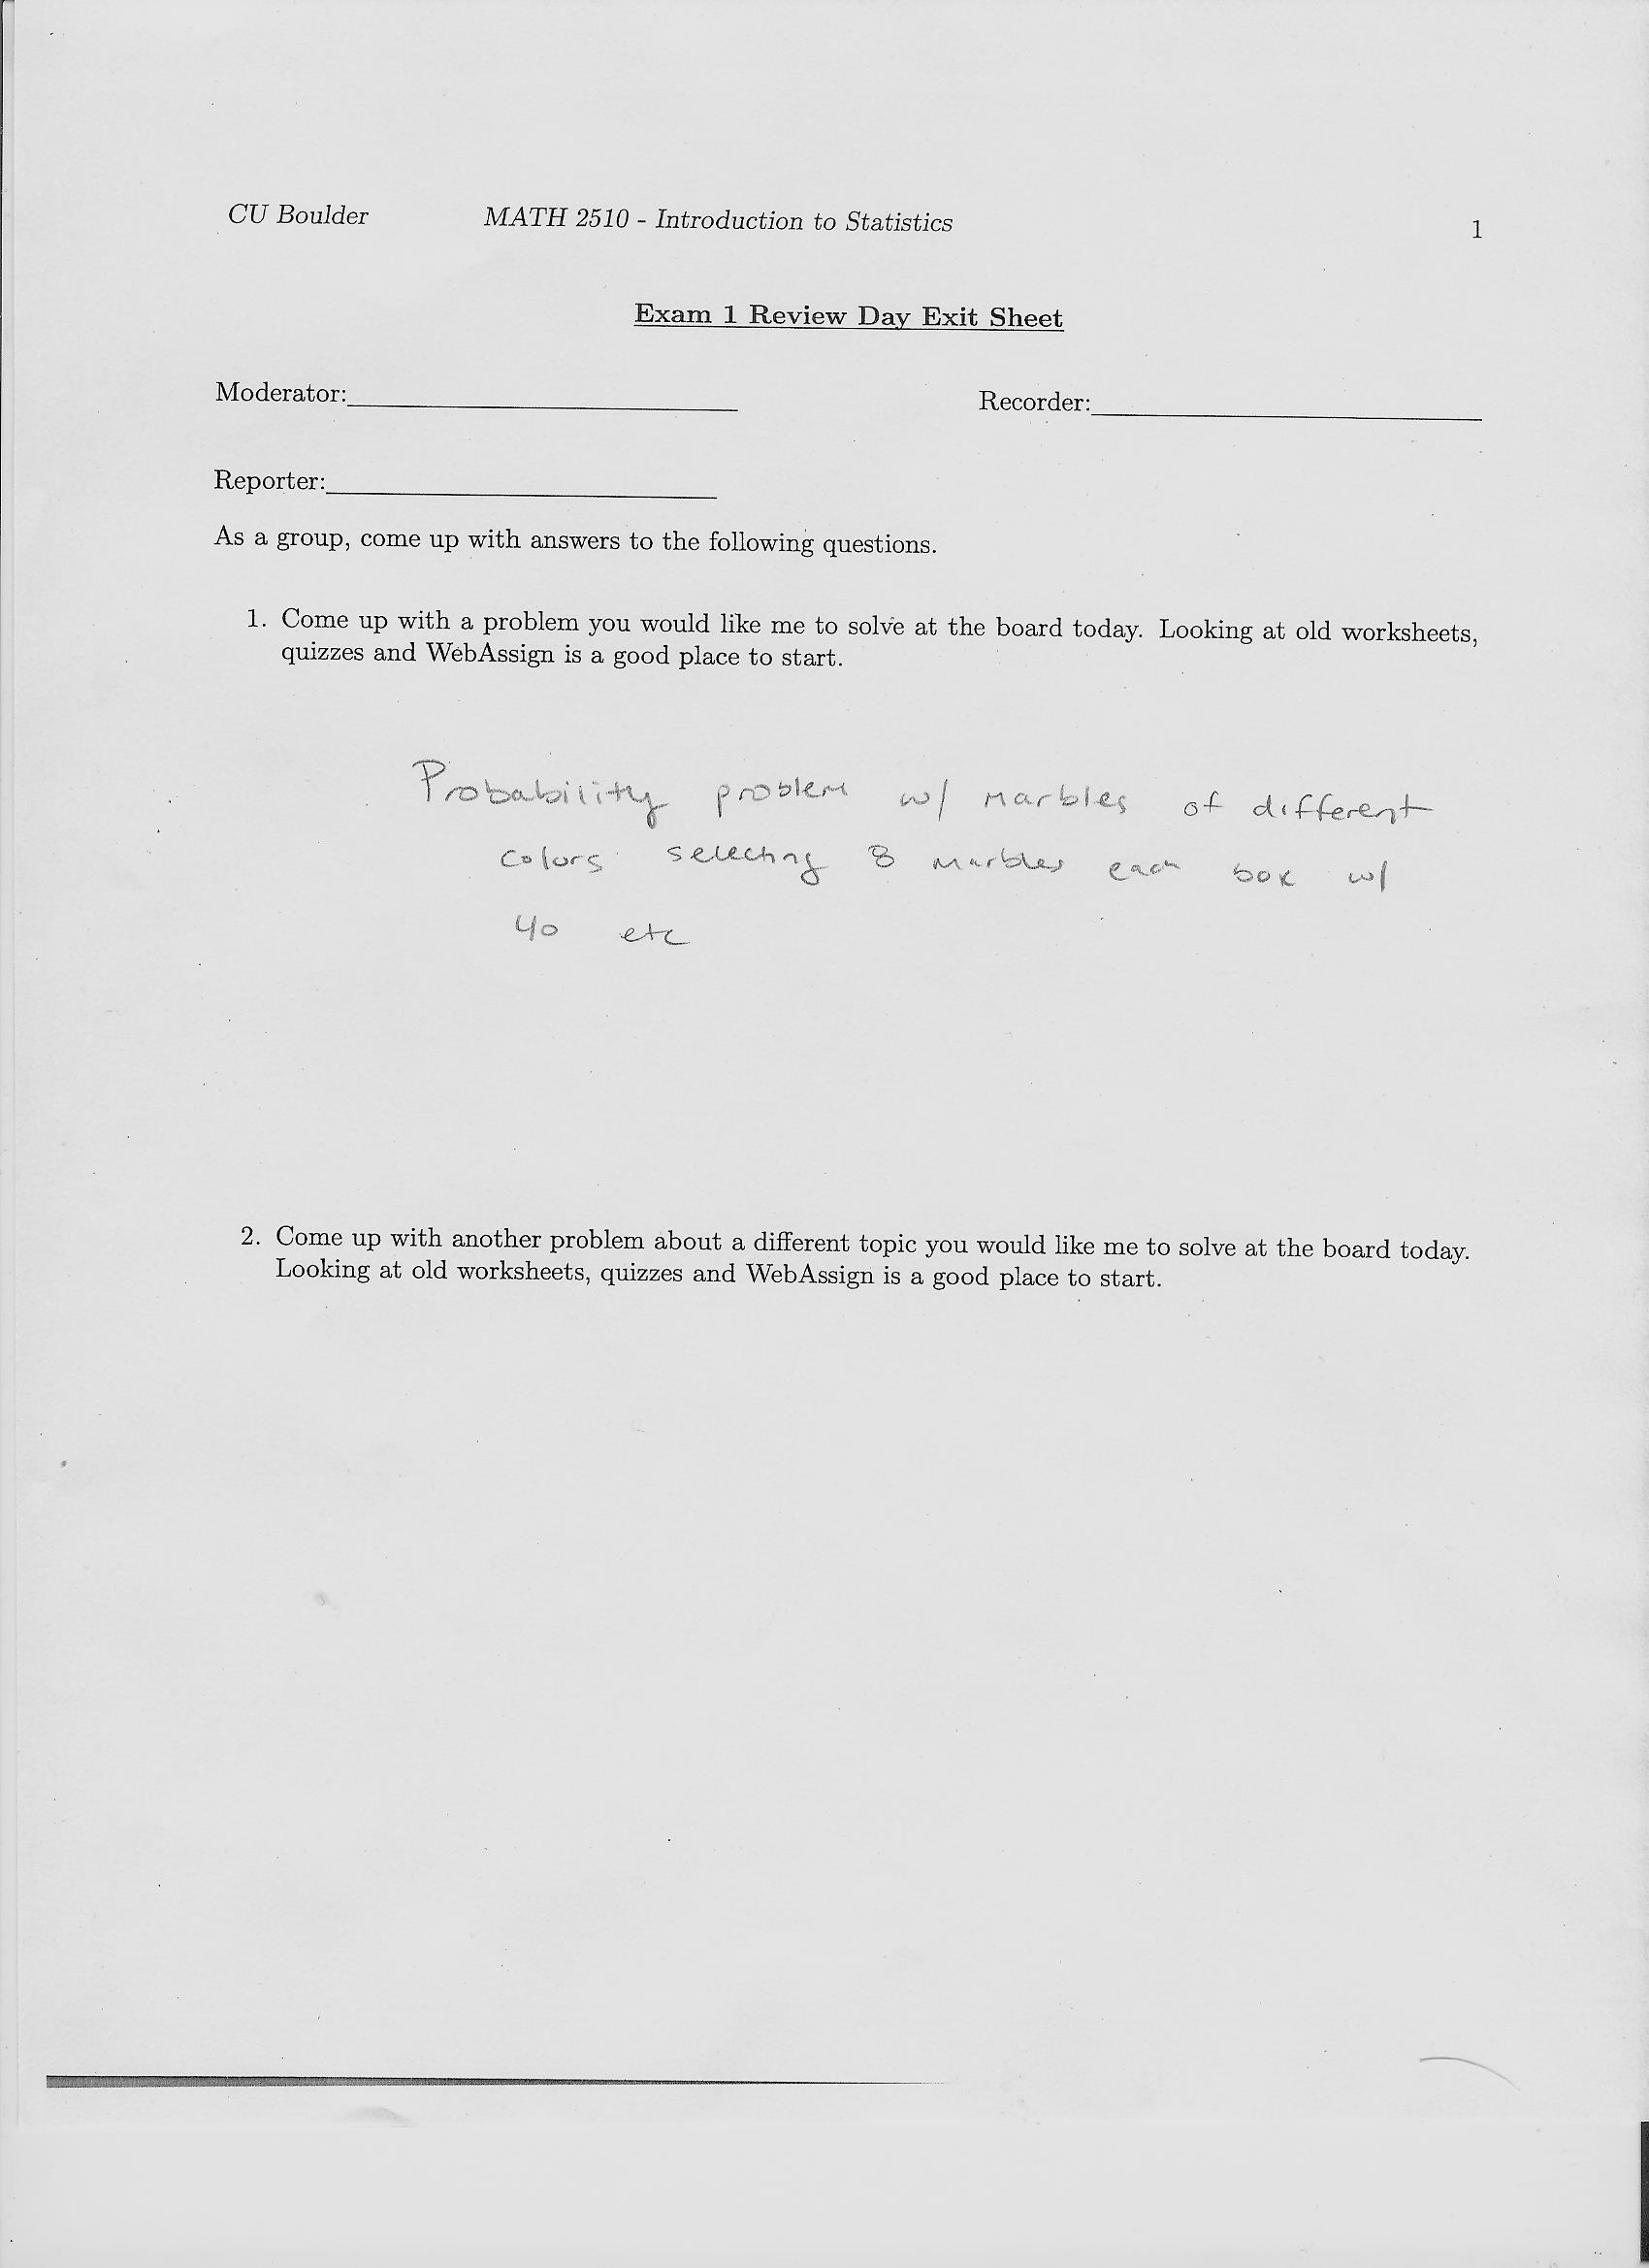
\includepdf{Exam1Exitsheet2.jpg}

\includepdf[pages=2]{2510-Quiz5-SS18-A}

\begin{center}
\textbf{\underbar{Exam 1 Review Day Exit Sheet}}
\end{center}

Moderator:{\underbar{\hspace{2in}}} \hfill  Recorder:{\underbar{\hspace{2in}} 

\bigskip

Reporter:{\underbar{\hspace{2in}}

As a group, come up with answers to the following questions.

\begin{enumerate} 

\item Come up with a problem you would like me to solve at the board today. Looking at old worksheets, quizzes and WebAssign is a good place to start.

{\answer I believe this is referencing Question 2 from Quiz 5, which is included before this page.

a.) The binomial model cannot be used for this because we are sampling without replacement. This leads to dependent trials (the probability of a success in future trials is dependent on the outcomes of previous trials) and we must have independent trials for the binomial model.

b.) The binomial model can be used because the trials are independent and the probability of a success (drawing a red marble) is constant and all other outcomes (drawing a purple or green) are treated as a failure.

So the answer is $\mbox{\texttt{binompdf}}(8, 14/40, 1) \approx 0.1372624$.

c.) The binomial model cannot be used for this because no matter what color(s) you deem a ``success'', you will need to either distinguish between types of success or types of failure. In other words, any decision leads to independent trials with more than 2 outcomes.}

\item Come up with another problem about a different topic you would like me to solve at the board today. Looking at old worksheets, quizzes and WebAssign is a good place to start. 

\end{enumerate}

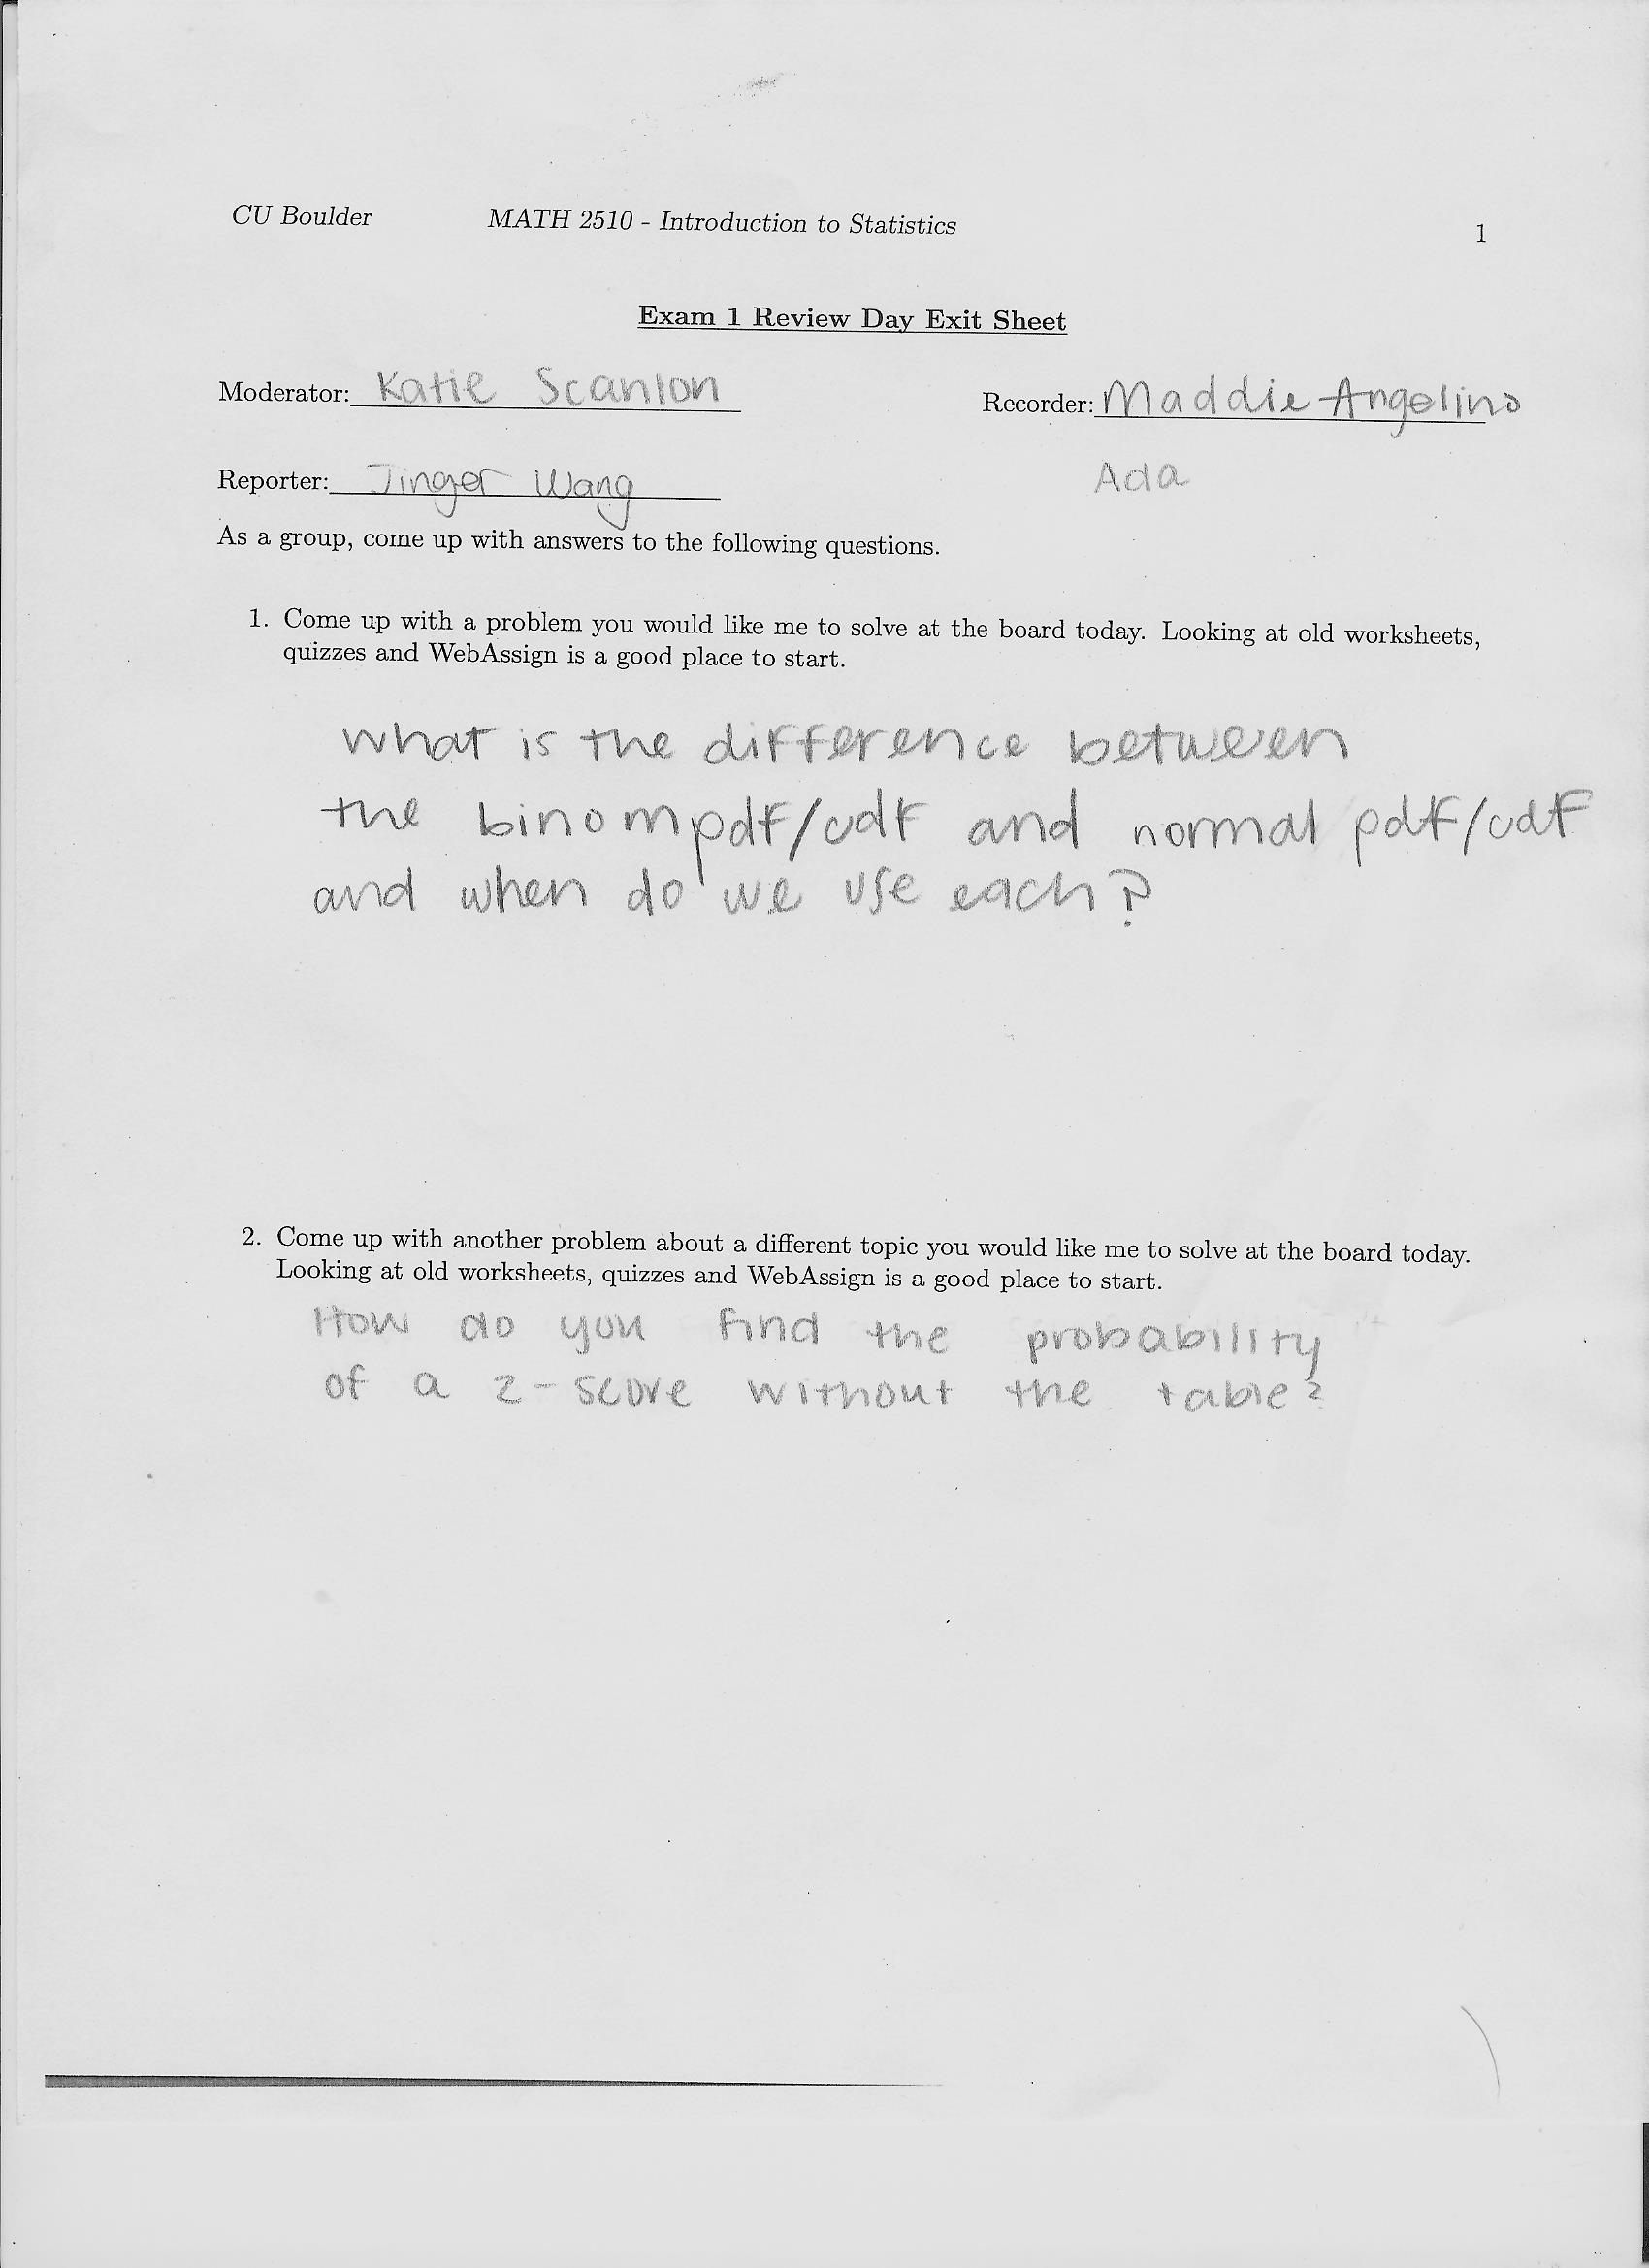
\includepdf{Exam1Exitsheet3.jpg}

\begin{center}
\textbf{\underbar{Exam 1 Review Day Exit Sheet}}
\end{center}

Moderator:{\underbar{\hspace{2in}}} \hfill  Recorder:{\underbar{\hspace{2in}}}

\bigskip

Reporter:{\underbar{\hspace{2in}}

As a group, come up with answers to the following questions.

\begin{enumerate} 

\item Come up with a problem you would like me to solve at the board today. Looking at old worksheets, quizzes and WebAssign is a good place to start.

{\answer The difference between \texttt{binompdf} and \texttt{binomcdf} is the type of events these functions compute the probability of in the binomial model. The function \texttt{binompdf} gives the probability of \textit{exactly} $x$ many successes $P(X=x)$ and \texttt{binomcdf} gives the probability of \textit{at most} $x$ many successes $P(X\leq x)$. In other words, 
$$\mbox{\texttt{binomcdf}}(10,0.4,2) = \mbox{\texttt{binompdf}}(10,0.4,0) + \mbox{\texttt{binompdf}}(10,0.4,1) + \mbox{\texttt{binompdf}}(10,0.4,2)$$

The function \texttt{normalpdf} gives the height of a normal distribution and is of no use in this class. The function \texttt{normalcdf} is used to compute the probability that a normally distribution object falls between a lower bound and upper bound.}

\item Come up with another problem about a different topic you would like me to solve at the board today. Looking at old worksheets, quizzes and WebAssign is a good place to start. 

{\answer The short answer is you use $\texttt{normalcdf}(LB, UB,\mu,\sigma)$ to compute the probability a normally distributed is between two numbers, $P(LB\leq x \leq UB)$. A $z$-table gives you $P(z\leq z_0)$, where you choose a value $z_0$ and $z$ is normally distributed with mean $0$ and standard deviation $1$.}
\end{enumerate}

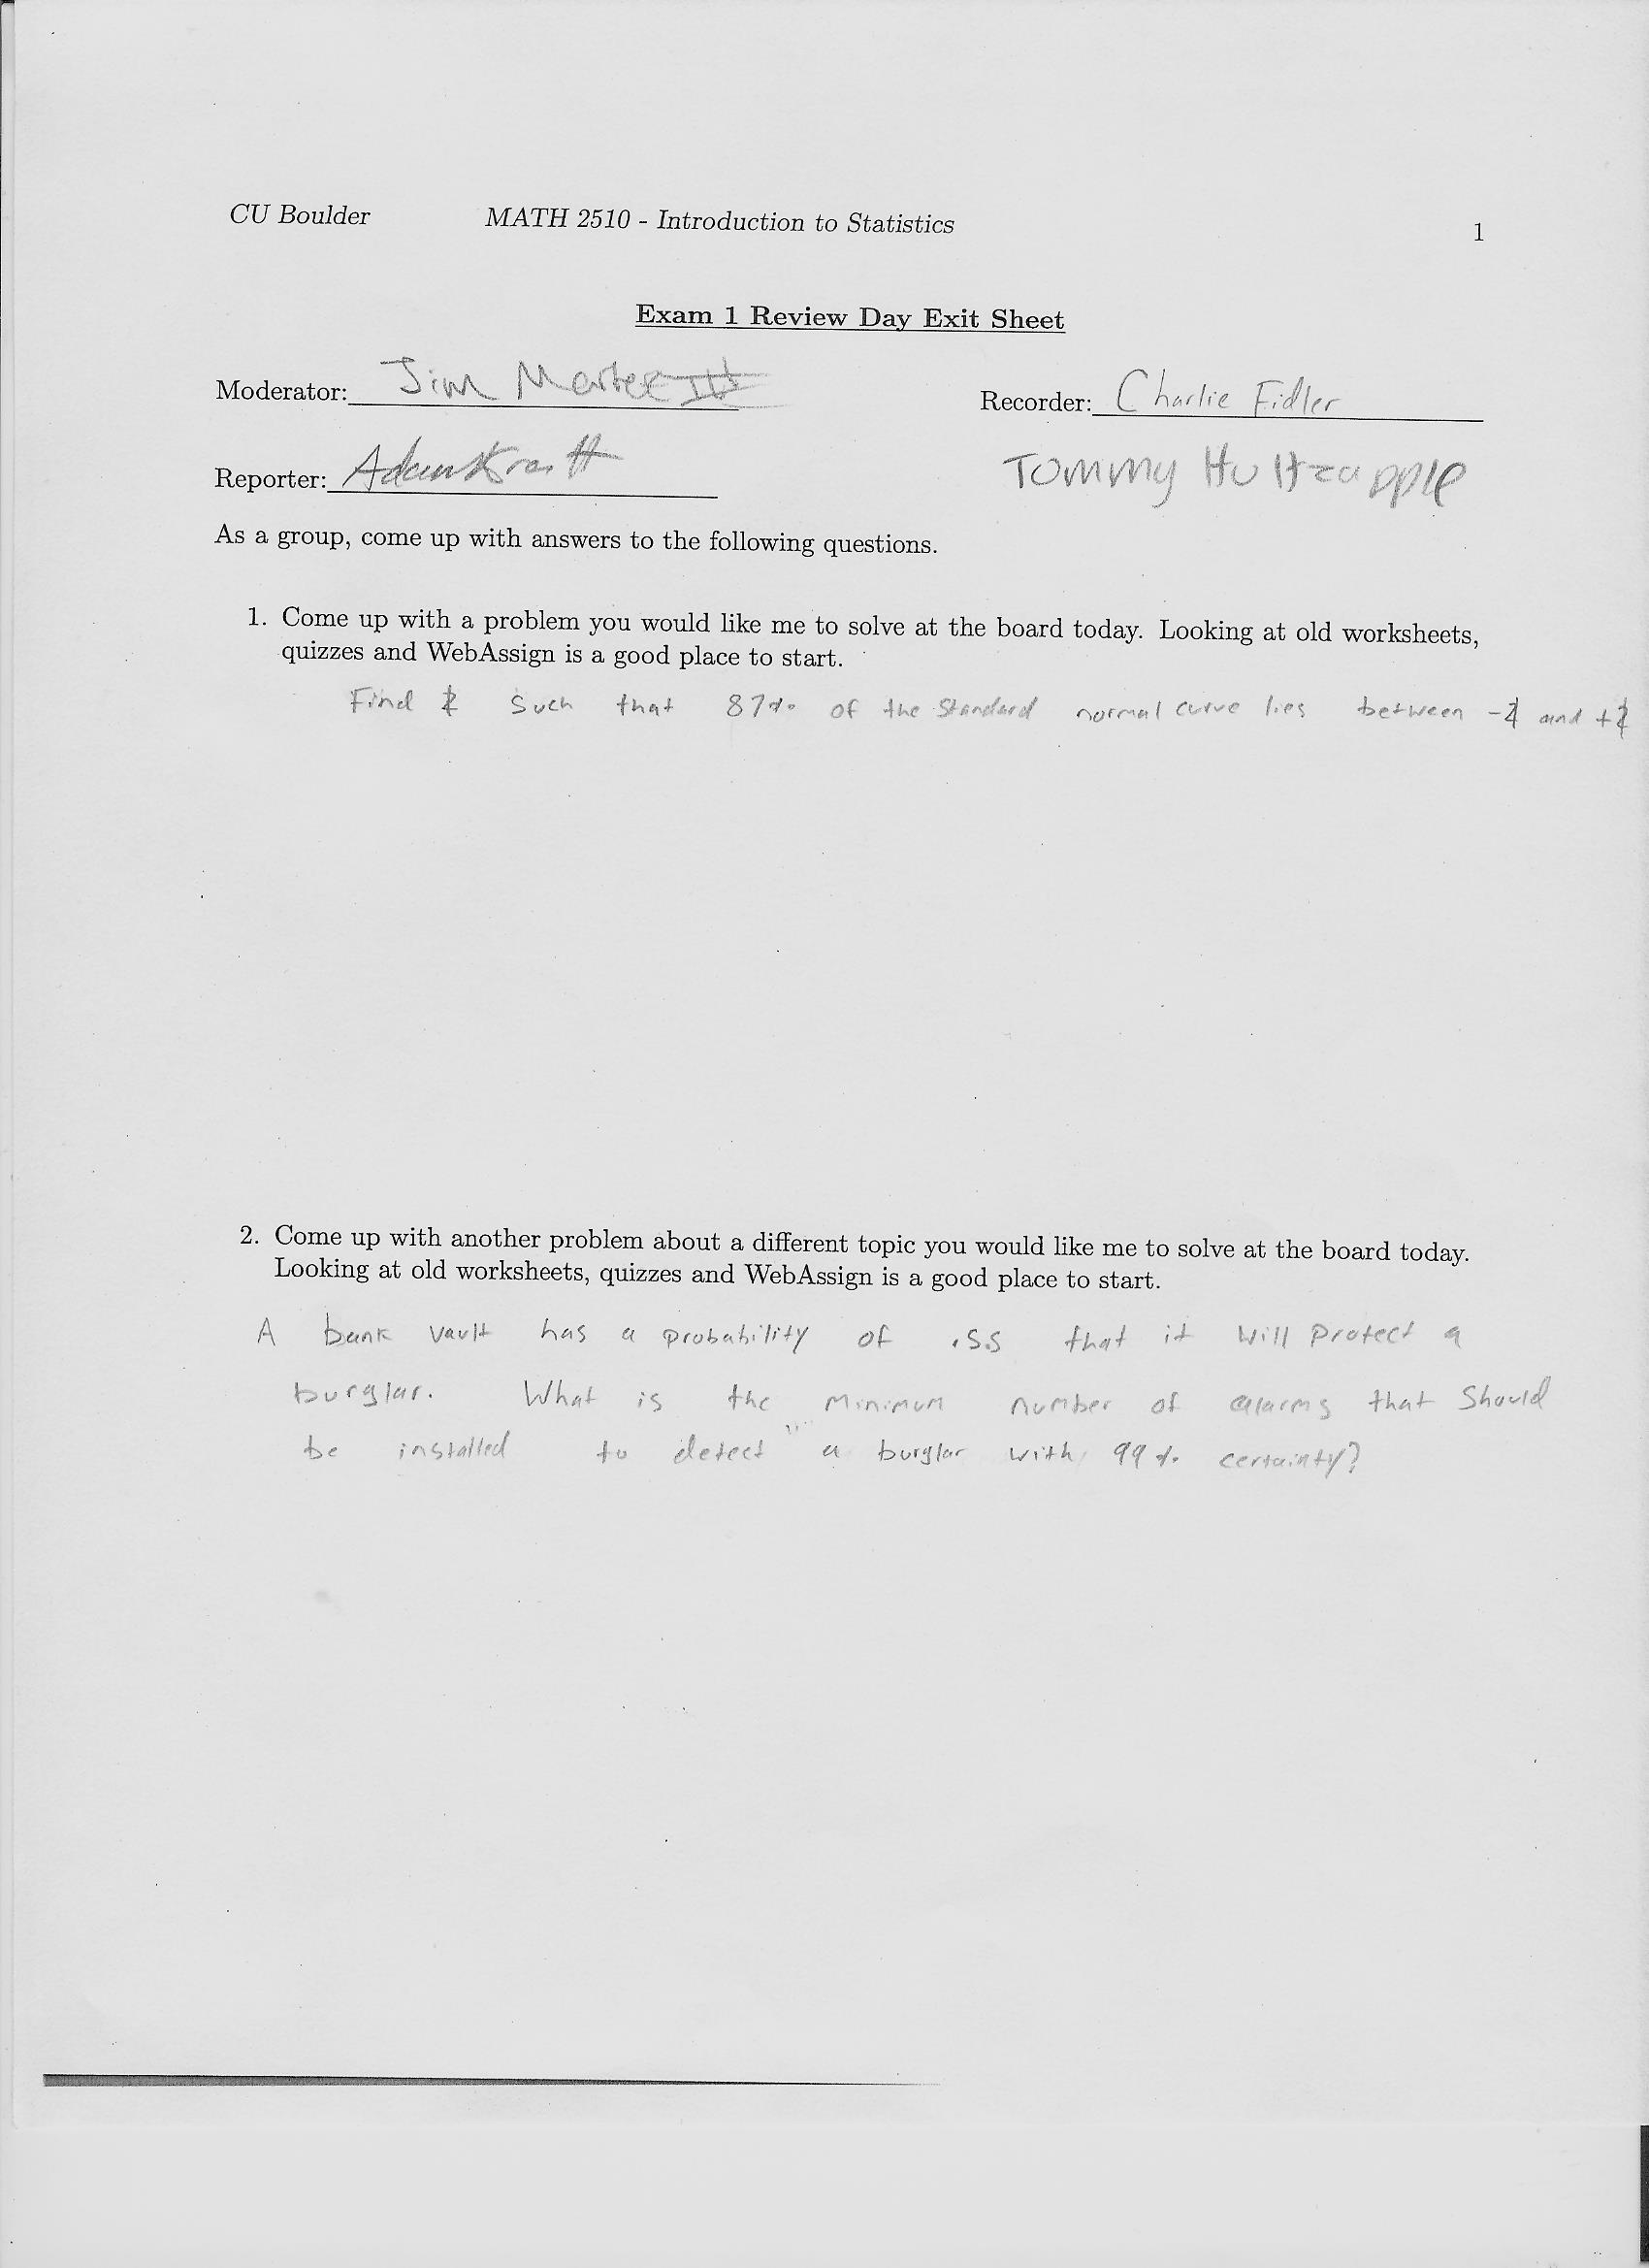
\includepdf{Exam1Exitsheet4.jpg}

\begin{center}
\textbf{\underbar{Exam 1 Review Day Exit Sheet}}
\end{center}

Moderator:{\underbar{\hspace{2in}}} \hfill  Recorder:{\underbar{\hspace{2in}}}

\bigskip

Reporter:{\underbar{\hspace{2in}}}

As a group, come up with answers to the following questions.

\begin{enumerate} 

\item Come up with a problem you would like me to solve at the board today. Looking at old worksheets, quizzes and WebAssign is a good place to start.

{\answer For this, we will use \texttt{invNorm} to find the answer. To use this function, we must determine the area to the left of the described $z$. Since the area between $-z$ and $z$ is 0.86, there is 0.14 outside of this region. Thus between $-\infty$ and $-z$, there is 0.07. Adding, we see there must be $0.07 + 0.86 = 0.93$ to the left of $z$.
$$z = \texttt{invNorm}(0.93,0,1) \approx 1.4758.$$ }

\item Come up with another problem about a different topic you would like me to solve at the board today. Looking at old worksheets, quizzes and WebAssign is a good place to start. 

{\answer Already answered!}
\end{enumerate}

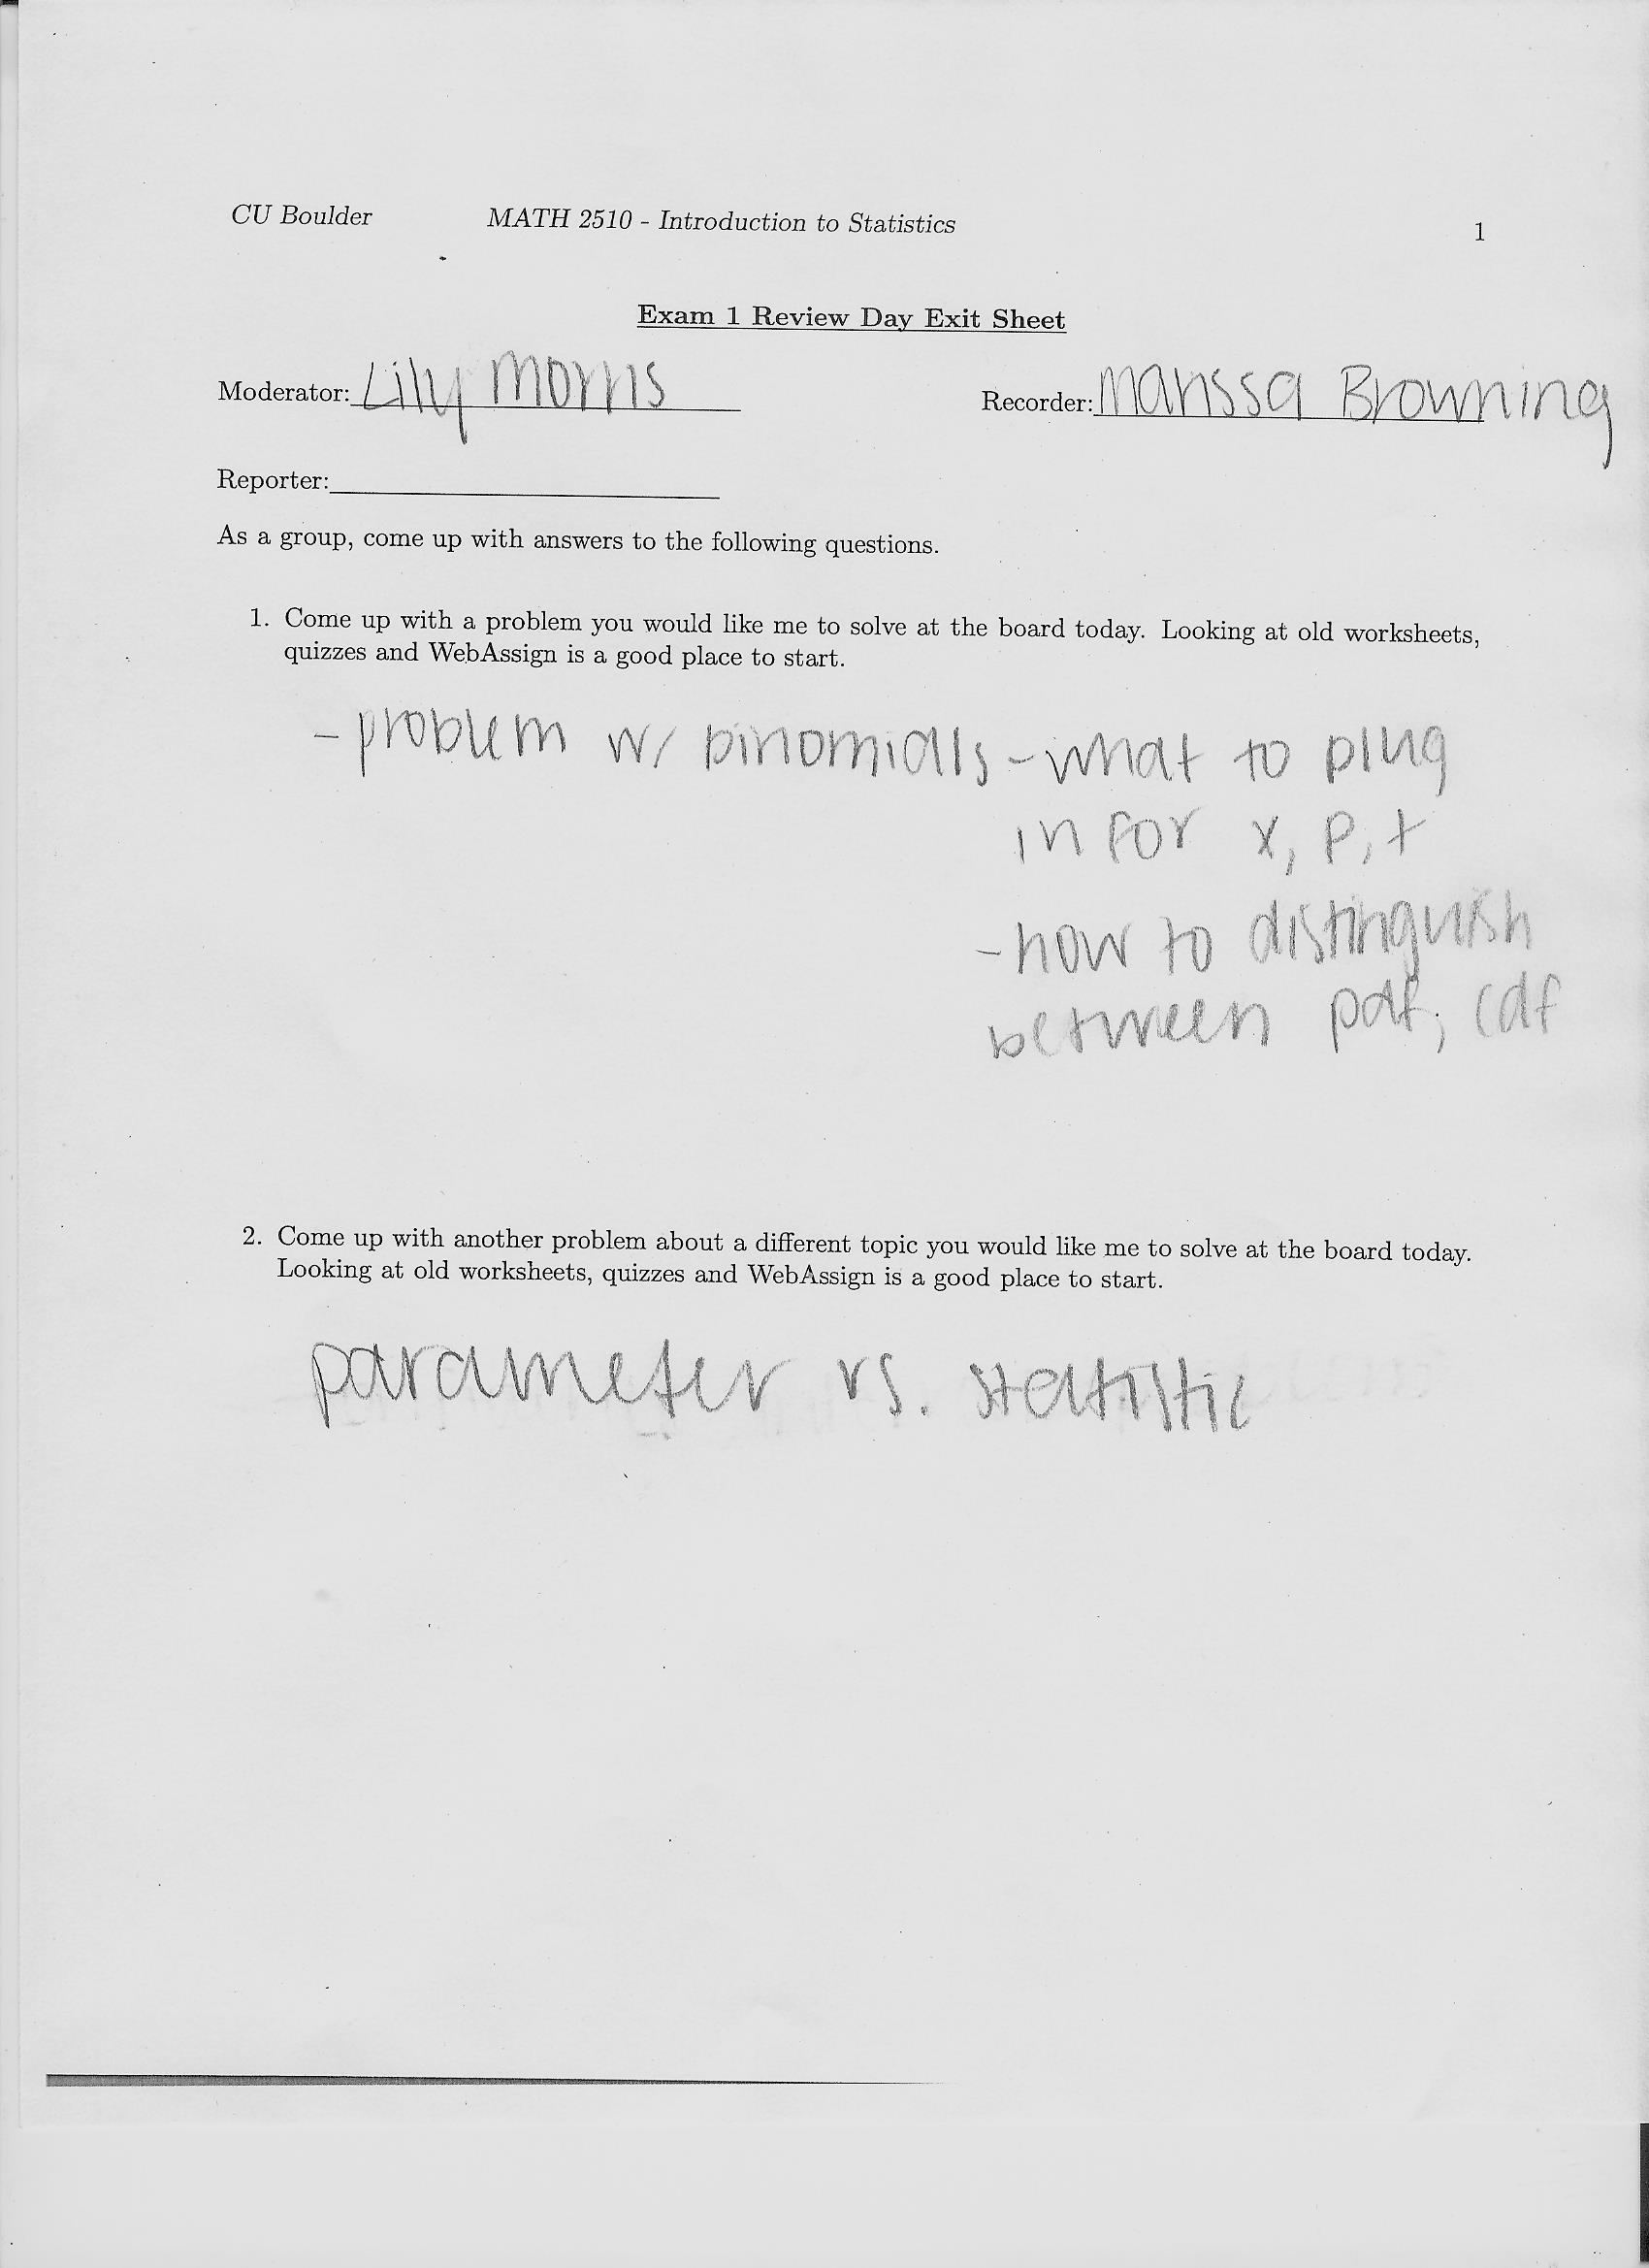
\includepdf{Exam1Exitsheet5.jpg}

\begin{center}
\textbf{\underbar{Exam 1 Review Day Exit Sheet}}
\end{center}

Moderator:{\underbar{\hspace{2in}}} \hfill  Recorder:{\underbar{\hspace{2in}}}

\bigskip

Reporter:{\underbar{\hspace{2in}}}

As a group, come up with answers to the following questions.

\begin{enumerate} 

\item Come up with a problem you would like me to solve at the board today. Looking at old worksheets, quizzes and WebAssign is a good place to start.

{\answer I already covered the difference between the pdf and cdf functions for binomial.

As far as what to plug in for $x$, $p$ and $n$, these are usually described in the problem. $n$ is the number of trials (or times the experiment is performed), $p$ is the probability a trial ends in success and $x$ is the number of total successes one is looking for.

Since our calculator is limited, one common event we may try to find the probability of is (and I chose 8 randomly) $P(X \geq 8)$. 
\begin{align*}
P(X\geq 8) &= 1 - P(X<8) \\
&= 1 - P(X\leq 7) \\
&= 1- \texttt{binomcdf}(n,p,7)\end{align*}}

\item Come up with another problem about a different topic you would like me to solve at the board today. Looking at old worksheets, quizzes and WebAssign is a good place to start. 

{\answer A parameter is some kind of measurement of an entire population (for example, the mean height of every person in the world) and a statistic is some kind of measurement of a sample of that population (the mean height of people in Boulder county).

What we call the ``population'' is relative. That is, it does not need to be every possible thing (for example, we could take our population to be every person in Boulder county). The relationship is that a sample is a smaller collection of a population.

The point of statistics (the subject) is that we can take a small random sample of a population, take a measurement of that sample (an actual statistic) and infer the nature or value of the population (what the parameter is).}

\end{enumerate}

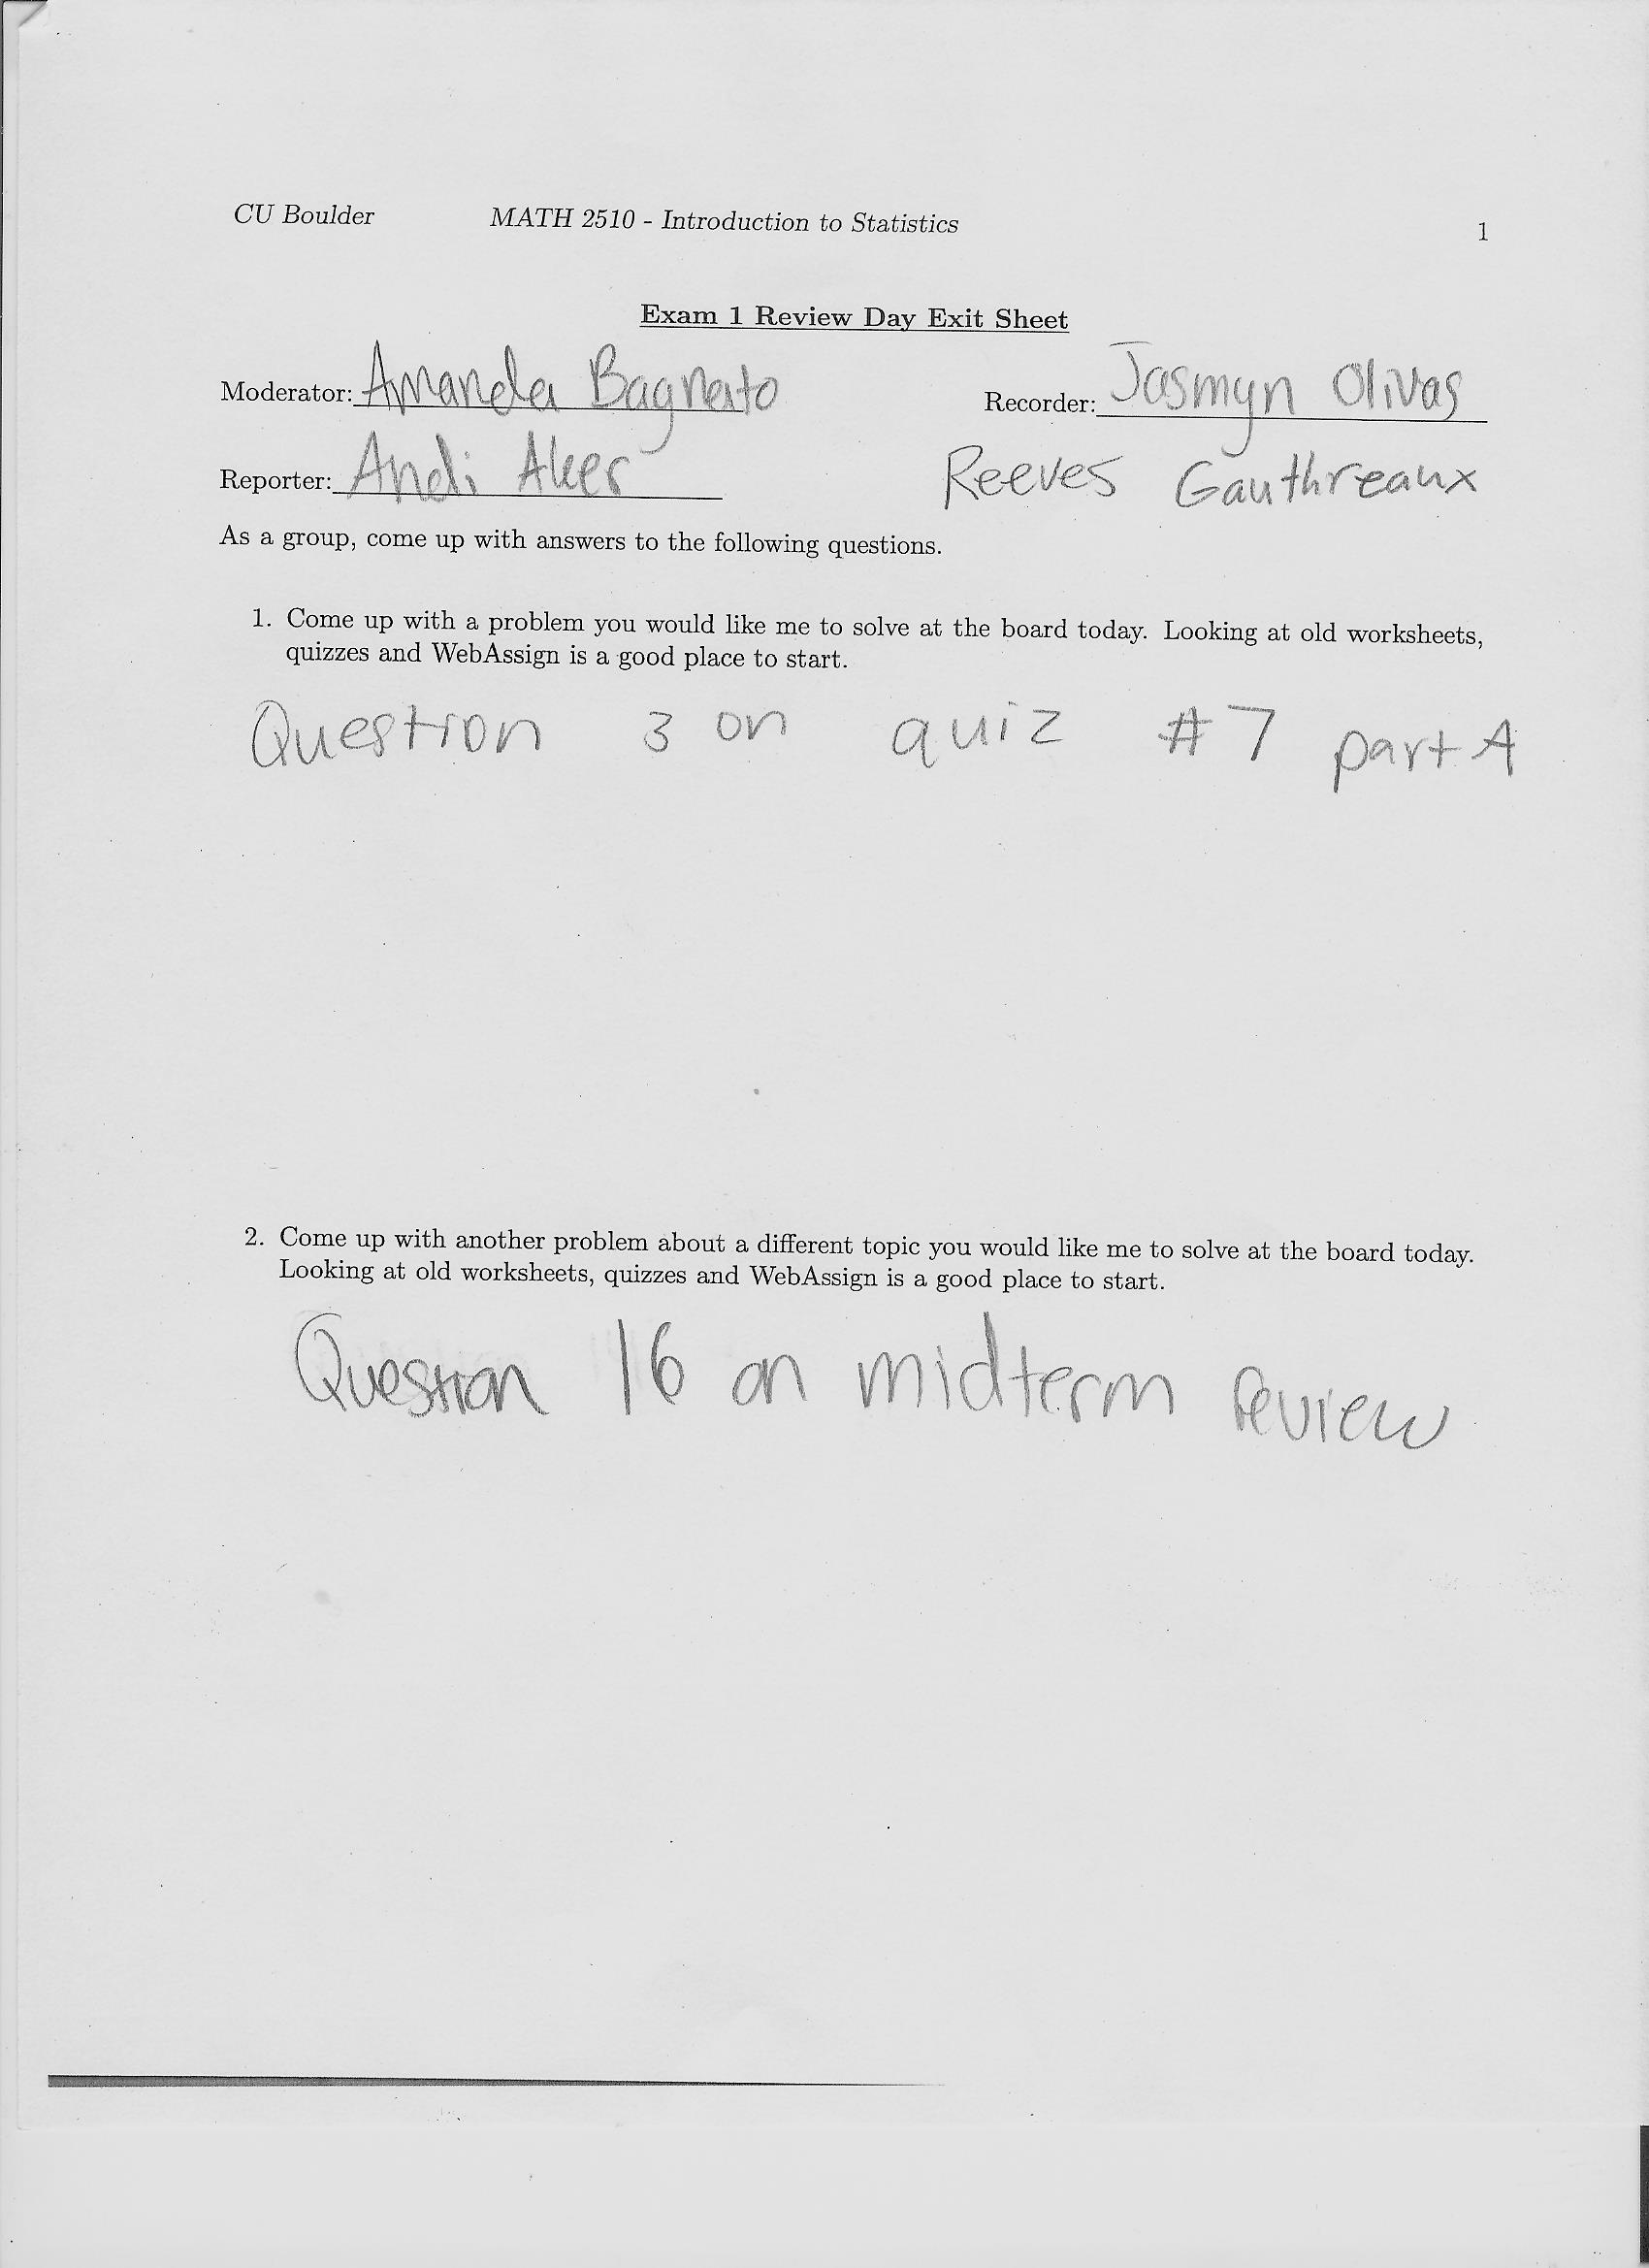
\includepdf{Exam1Exitsheet6.jpg}

\includepdf[pages=2]{2510-Quiz7-S18-A}

\begin{center}
\textbf{\underbar{Exam 1 Review Day Exit Sheet}}
\end{center}

Moderator:{\underbar{\hspace{2in}}} \hfill  Recorder:{\underbar{\hspace{2in}}}

\bigskip

Reporter:{\underbar{\hspace{2in}}}

As a group, come up with answers to the following questions.

\begin{enumerate} 

\item Come up with a problem you would like me to solve at the board today. Looking at old worksheets, quizzes and WebAssign is a good place to start.

{\answer The central limit theorem tells us, when the sample size is larger than 30, that sample means will follow a normal distribution. The mean of this sampling distribution will be the same as the mean of the population (15.17) and the standard deviation will be the population standard deviation divided by the square root of sample size ($\sigma/\sqrt{n} = 4.12/\sqrt{100} = 0.412$.)}

\item Come up with another problem about a different topic you would like me to solve at the board today. Looking at old worksheets, quizzes and WebAssign is a good place to start. 

{\answer Check the solutions that were posted to D2L!}

\end{enumerate}

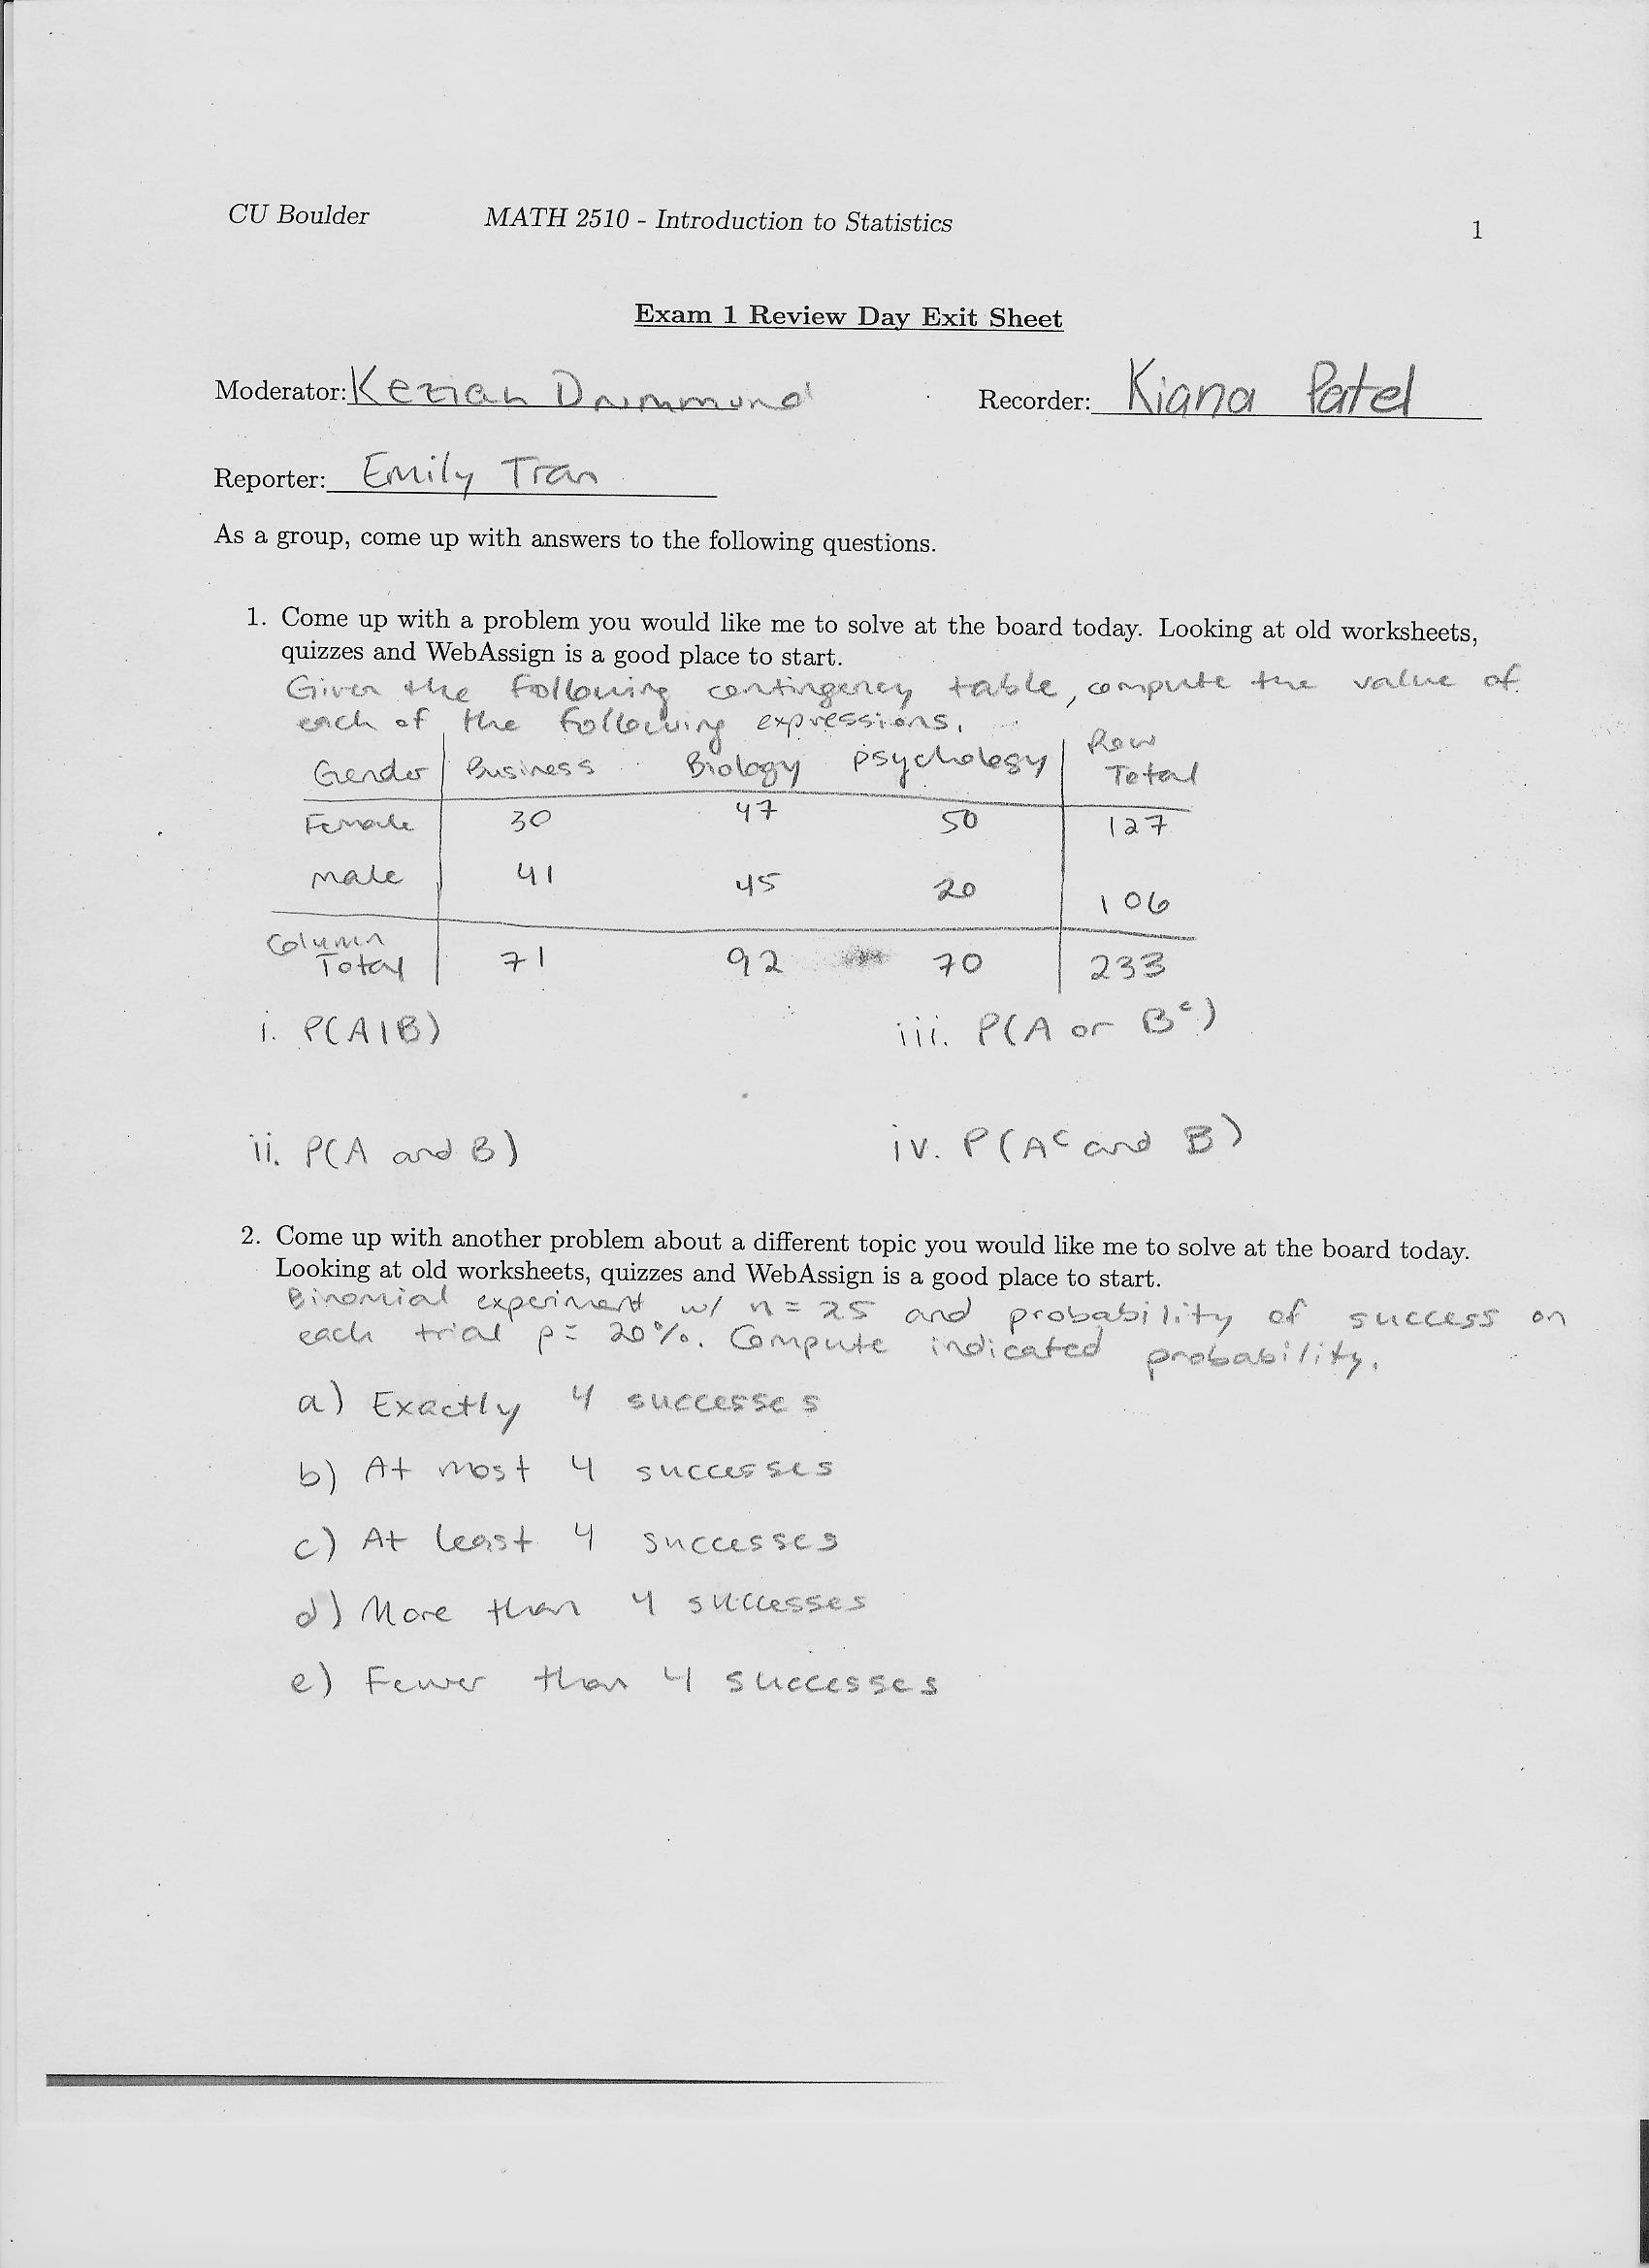
\includepdf{Exam1Exitsheet7.jpg}

\begin{center}
\textbf{\underbar{Exam 1 Review Day Exit Sheet}}
\end{center}

Moderator:{\underbar{\hspace{2in}}} \hfill  Recorder:{\underbar{\hspace{2in}}}

\bigskip

Reporter:{\underbar{\hspace{2in}}}

As a group, come up with answers to the following questions.

\begin{enumerate} 

\item Come up with a problem you would like me to solve at the board today. Looking at old worksheets, quizzes and WebAssign is a good place to start.

{\answer Let event A be "male student" and event B "biology major"
    \begin{enumerate}
        \item This is the percentage of biology majors that are males, $45/92$.
        \item This is the percentage of students that are male, biology majors $45/233$.
        \item This is the percentage of students that are either male or not biology majors $186/233$.
        \item This is the percentage of students that are not male (to be interpreted as 'females' I guess) that are biology majors, $47/233$.
    \end{enumerate}}

\item Come up with another problem about a different topic you would like me to solve at the board today. Looking at old worksheets, quizzes and WebAssign is a good place to start. 

{\answer \begin{enumerate}
    \item Since we want exactly 4 successes, $\texttt{binompdf}(25, 0.2, 4) \approx 0.18668$
    \item At most 4 is "4 or fewer" $\texttt{binomcdf}(25,0.2,4) \approx 0.42067$
    \item At least 4 is "4 or more", which has complement "3 or less", $1-\texttt{binomcdf}(25, 0.2, 3) \approx 0.766$
    \item More than 4 is "5 or more", which has complement "4 or less",
    $1-\texttt{binomcdf}(25,0.2,4)\approx 0.57933$.
    \item Fewer than 4 is "3 or less", $\texttt{binomcdf}(25,0.2,3) \approx 0.23399$.
    \end{enumerate}}

\end{enumerate}

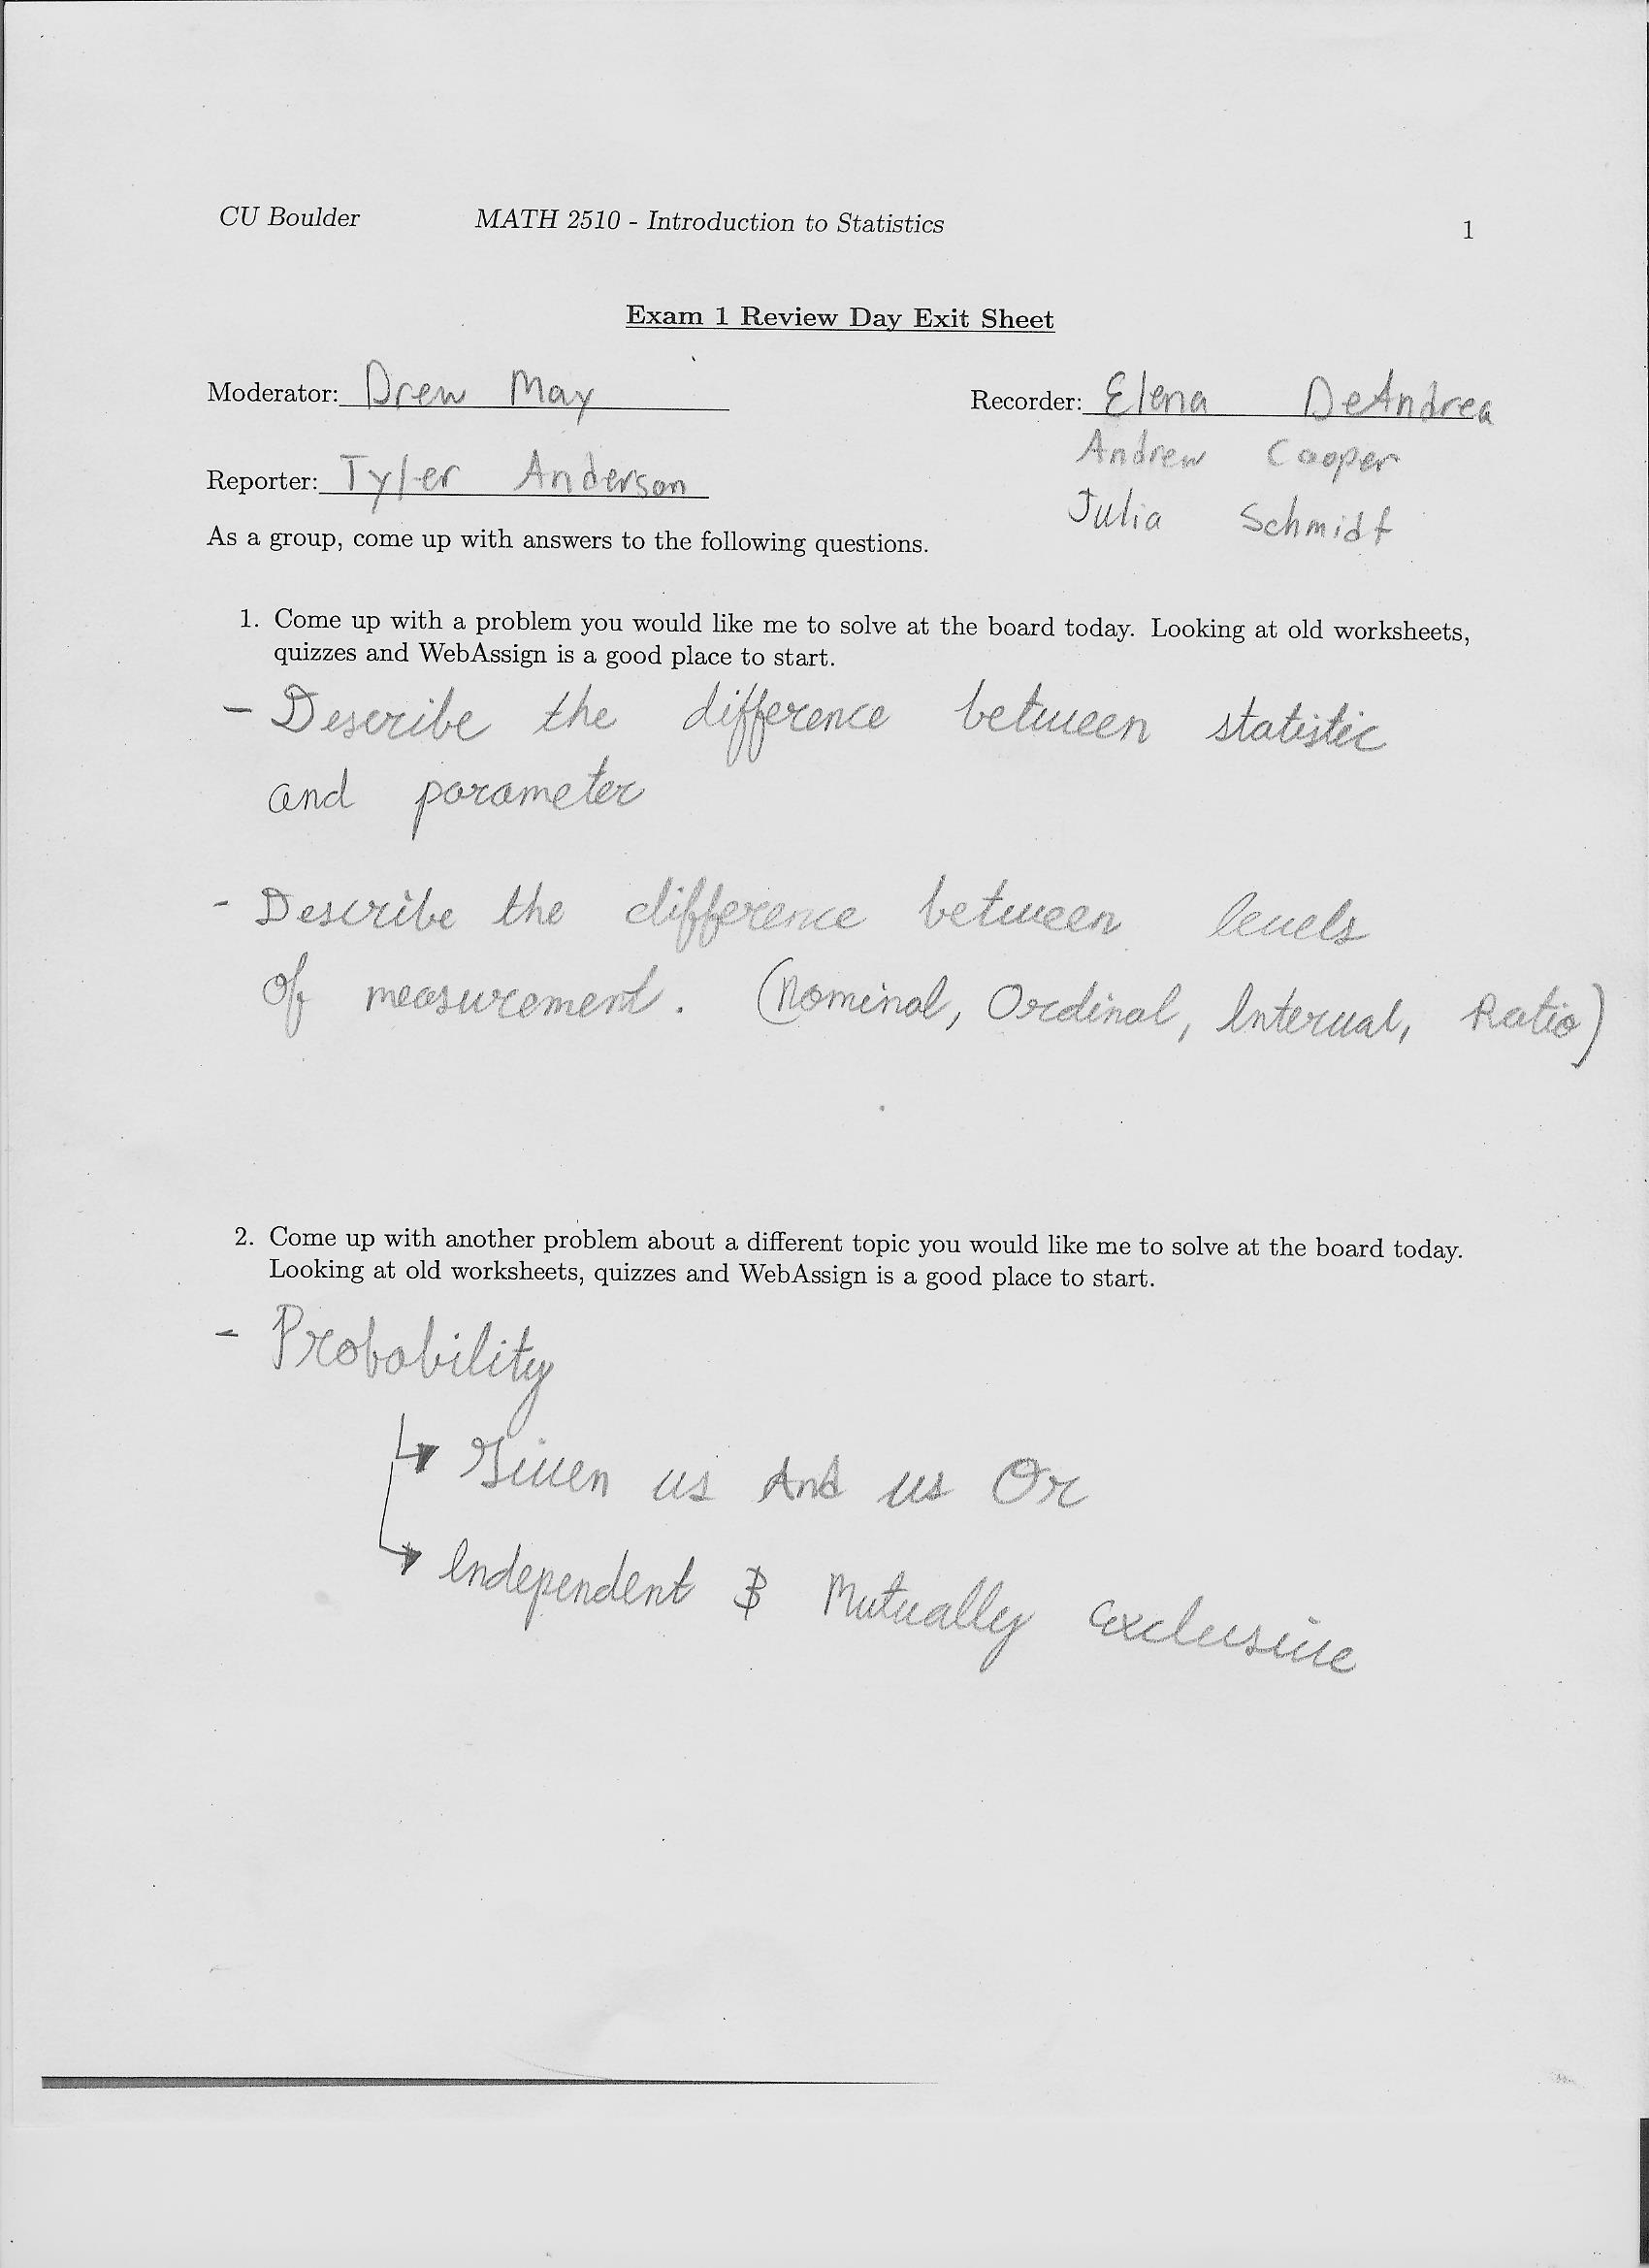
\includepdf{Exam1Exitsheet8.jpg}

\begin{center}
\textbf{\underbar{Exam 1 Review Day Exit Sheet}}
\end{center}

Moderator:{\underbar{\hspace{2in}}} \hfill  Recorder:{\underbar{\hspace{2in}}}

\bigskip

Reporter:{\underbar{\hspace{2in}}}

As a group, come up with answers to the following questions.

\begin{enumerate} 

\item Come up with a problem you would like me to solve at the board today. Looking at old worksheets, quizzes and WebAssign is a good place to start.

{\answer I've already answered the first question, so onto the second:

Nominal data is data for which there is no meaningful order. That is, the order in which one puts the data does not convey the idea of more or less of the quality (or quantity being measured. Examples include last names, Jersey numbers, and color.

Ordinal data is for data in which there is an order which conveys more or less of something. However, the difference (subtracting values from others) between points does not make sense. My favourite examples are shirt sizes (large, small, etc.) and letter grades.

Interval data is quantitative, ordinal data in which differences is meaningful. However, the value of 0 does not reflect the absence of the quantity. Temperature in Fahrenheit is a great example.

Ratio data is interval data in which 0 does reflect the absence of the quantity. Height, weight, velocity are all good examples.}

\item Come up with another problem about a different topic you would like me to solve at the board today. Looking at old worksheets, quizzes and WebAssign is a good place to start. 

{\answer Not sure about the first part, but hopefully the previous questions address this.

Independent means that $P(A \mbox{ and } B) = P(A) \cdot P(B)$. It is equivalent (assuming probabilities are non-zero) to $P(A) = P(A|B)$ or $P(B) = P(B|A)$.

Mutually exclusive means that events $A$ and $B$ share no common outcome. For example, the events "a card is a spade" and "a card is a heart" are mutually exclusive. As a consequence, mutually exclusive events have $P(A \mbox{ and } B) = 0$}

\end{enumerate}
\end{document}